\documentclass[dvipdfmx]{jarticle}
\usepackage{graphicx}
\usepackage{here}
\usepackage{ascmac}
\usepackage{amsmath,amssymb}
\usepackage[margin=20mm]{geometry}
\usepackage{listings,jvlisting} %日本語のコメントアウトをする場合jvlisting(もしくはjlisting)が必要
%ここからソースコードの表示に関する設定
\lstset{
  basicstyle={\ttfamily},
  identifierstyle={\small},
  commentstyle={\smallitshape},
  keywordstyle={\small\bfseries},
  ndkeywordstyle={\small},
  stringstyle={\small\ttfamily},
  frame={tb},
  breaklines=true,
  columns=[l]{fullflexible},
  numbers=left,
  xrightmargin=0zw,
  xleftmargin=3zw,
  numberstyle={\scriptsize},
  stepnumber=1,
  numbersep=1zw,
  lineskip=-0.5ex
}
\setcounter{tocdepth}{4}
\pagestyle{empty}
\begin{document}
\title{計算機科学実験及演習4 データベース 課題2}
\author{1029-32-6611 山田裕晃}
\maketitle

\section{概要}
課題1で作成したER図について関係スキーマを設計する。
設計した各関係スキーマに対して自明でない関数従属性の集合を求め、もし自明でない関数従属性が存在しなければ存在するようにER図を変更する。
各関数従属性がなぜ成立するのかを文章で説明する。

さらに,自明でないかつ関数従属性でない多値従属性が存在する場合はそれを示し,各多値従属性がなぜ成立するのかを文章で説明する。

\section{関係スキーマの導出}
課題1で作成したER図をもとに、関係スキーマを導出する。以下に、課題1で作成したER図を再掲する。
\begin{figure}[H]
  \centering
  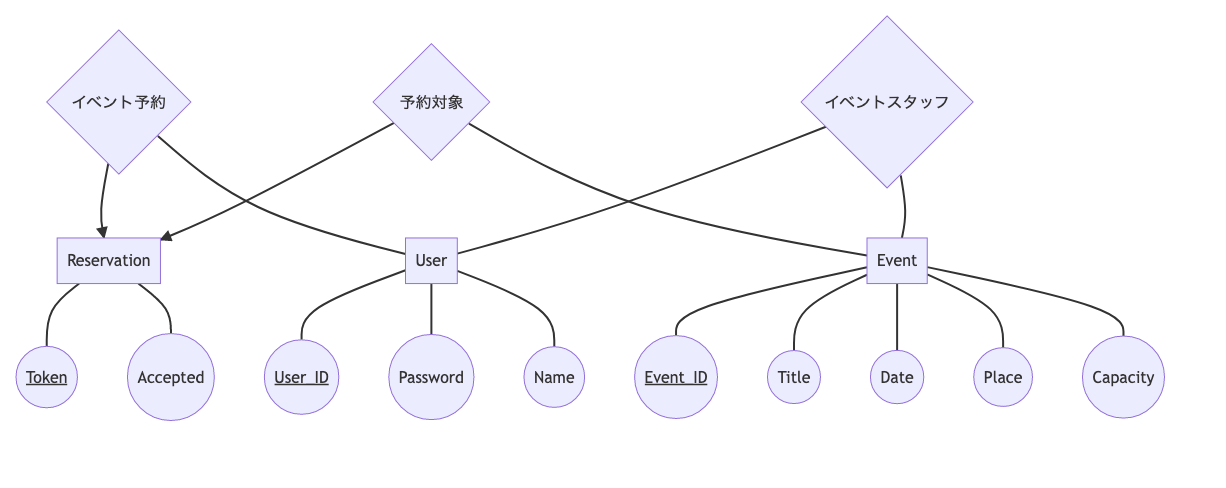
\includegraphics[scale=0.4]{ermodel.png}
  \caption{ER図}
\end{figure}

予約(Reservation)について、関係「予約」を定義する。
「予約」の属性であるトークン(Token)と受付状態(Accepted)を「予約」の属性とする。主キーはトークンとする。

ユーザー(User)について、関係「ユーザー」を定義する。
「ユーザー」の属性であるユーザーID(UserID)とパスワード(Password)と名前(Name)を「イベントスタッフ」の属性とする。主キーはユーザーIDとする。

イベントについて、イベントとユーザとの間で関係「予約対象イベント」を定義する。
「イベント」の属性であるイベントID(EventID)とイベント名(Title)と開催日時(Date)と開催場所(Place)と定員(Capacity)を属性として持つ。

ここで、各関連集合について、関連集合の持つ属性と参加している実体集合の主キーを合わせたものを各関係のスキーマとする。

求めた関係スキーマを以下に記す。

\begin{description}
  \item[予約] \underline{トークン}, ユーザーID, イベントID, 受付状態
  \item[ユーザー] \underline{ユーザーID}, \underline{参加イベントID}, 名前, パスワード
  \item[イベント] \underline{イベントID}, \underline{スタッフユーザーID}, イベント名, 開催日時, 開催場所, 定員 
\end{description}

このままでは非常に冗長かつ更新不整合の問題が生じる可能性が高い。

\section{自明でない関数従属性の導出}
自明でない関数従属性は以下の通りである。
\begin{itemize}
  \item {トークン} $\rightarrow$ {ユーザーID}
  \item {トークン} $\rightarrow$ {イベントID}
  \item {トークン} $\rightarrow$ {受付状態}
\end{itemize}
これらは、トークンが実体集合「予約」の主キーであることより明らかである。
\begin{itemize}
  \item {ユーザーID} $\rightarrow$ {名前}
  \item {ユーザーID} $\rightarrow$ {パスワード}
\end{itemize}
これらは、トークンが実体集合「ユーザー」の主キーであることより明らかである。
\begin{itemize}
  \item {イベントID} $\rightarrow$ {イベント名}
  \item {イベントID} $\rightarrow$ {開催日時}
  \item {イベントID} $\rightarrow$ {開催場所}
  \item {イベントID} $\rightarrow$ {定員}
\end{itemize}
これらは、トークンが実体集合「イベント」の主キーであることより明らかである。

\section{多値従属性の確認}
以下の自明かつ関数従属性でない多値従属性が存在する。
\begin{itemize}
  \item {ユーザーID} $\rightarrow \rightarrow$ {参加イベントID}
\end{itemize}
ユーザーIDと参加イベントIDからなる関係とユーザーID, 名前, パスワードからなる関係を自然結合することで関係「ユーザー」が得られるため。
\begin{itemize}
  \item {イベントID} $\rightarrow \rightarrow$ {スタッフユーザーID}
\end{itemize}
イベントIDとスタッフユーザーIDからなる関係とイベントID, イベント名, 開催日時, 開催場所, 定員からなる関係を自然結合することで関係「イベント」が得られるため。

\end{document}